% \titleformat{\chapter}[block]
% {\filcenter\bfseries\Huge}
% {\xrfill[0.4ex]{5pt}\ \thechapter.\ \xrfill[0.4ex]{5pt}}
% {0pt}
% {\xrfill[0.4ex]{5pt}\ \MakeUppercase{#1}\ \xrfill[0.4ex]{5pt}}

\chapter*{Chapter 3}

\markboth{Sprint 1 : Application Skeleton }{3 Sprint 1 : Application Skeleton} %pour afficher l'entete
 \addcontentsline{toc}{chapter}{3 Sprint 1 : Application Skeleton}



\setcounter{chapter}{3}
\setcounter{section}{0}
\setcounter{table}{0} 
\setcounter{figure}{0} 


\etocsettocstyle{\subsection*{Plan}}{}
\vspace{0.25cm}

\setcounter{tocdepth}{1}
\headrule{
\vspace{0.5cm}

\begin{center}
    \textsc{\textbf {\Huge Sprint 1 : Application Skeleton}} 
\end{center}
}
\headrule


\localtableofcontents
\newpage






\section*{Introduction}
After having a good understanding of the project scope and requirements in the previous chapter.
In this chapter, we will tackle the realisation of  the first sprint of our project which handles the development of the core functionalities of the application like configuration,navigation and authentication . We will cover the planning and analysis of this sprint also we will go through the  implementation and testing and finally showcasing the artifacts .

\section{Sprint 1 Backlog}
The sprint backlog is a detailed list of tasks and user stories selected for completion within the current sprint, guiding the development team's work towards achieving the sprint goal. It serves as a dynamic, prioritized plan that evolves as the team progresses and new information emerges.
The table below describes the backlog of the firs sprint :



\begin{table}[H]
    % \centering
    \renewcommand{\arraystretch}{1.2}
    \setlength{\belowcaptionskip}{0.25cm}
 
   \begin{tabular}{|p{0.05\textwidth}|p{0.25\textwidth}|p{0.29\textwidth}|p{0.34\textwidth}|}
   \hline
   \textbf{ID}  &  \textbf{User Story } & \textbf{Description} & \textbf{Task} \\ \hline


   
   \begin{center}
       \textbf{1}
   \end{center} & \begin{center}
       As an administrator , I can enter my parameters to  configure the application 
   \end{center} &
   The administrator is capable to define the modules , access level and the constants used all over the application 
   & 

       \begin{itemize}[left=0pt, label={\textbf{\Huge .}}]
       % \renewcommand\labelitemi{\textbf{\Huge .}}
            \item Develop Constants service   
            \item Develop Modules service   
            \item Develop Init  service   

        \end{itemize} \\ \hline


   \begin{center}
       \textbf{2}
   \end{center} & \begin{center}
       As a  user, I want to navigate through the application modules 
   \end{center} &
   
  The  user can navigate between screens and interact with the application's modules  & 

       \begin{itemize}[left=0pt, label={\textbf{\Huge .}}]
            \item Develop a drawer navigator 
            \item Develop a tabs navigator
            \item Develop modules screens

        \end{itemize} \\ \hline
        % &&&&&&&&&&&&&&&&&&&&&&&&
   \begin{center}
       \textbf{3}
   \end{center} & \begin{center}
       As a  user, I want to authenticate to the application and access protected modules
   \end{center} &
   
  The  user can create an account , sign in to the app in order to access restricted modules,also he can reset his password  & 

       \begin{itemize}[left=0pt, label={\textbf{\Huge .}}]
            \item Develop application with navigation and protected pages
            \item Develop login interface
            \item Develop register interface
            \item Develop forget password interface
            \item Develop authentication backend
        \end{itemize} \\ \hline
\begin{center}
       \textbf{4}
\end{center} & \begin{center}
       As a registered user, I want to edit my account information
   \end{center} &Registered users can update their credentials such as name, phone number, password 
   &
   \begin{itemize}[left=0pt, label={\textbf{\Huge .}}]
            \item Develop user profile interface
            \item Implement the backend for managing user account 
            \end{itemize} \\ \hline
\end{tabular}
       \caption{Sprint 1 Backlog}
        \label{tab:my_label}
    
\end{table}
\section{Sprint 1 use case diagram}
From the user stories mentioned earlier we can define a use case diagram for this sprint.
\begin{figure}[H] 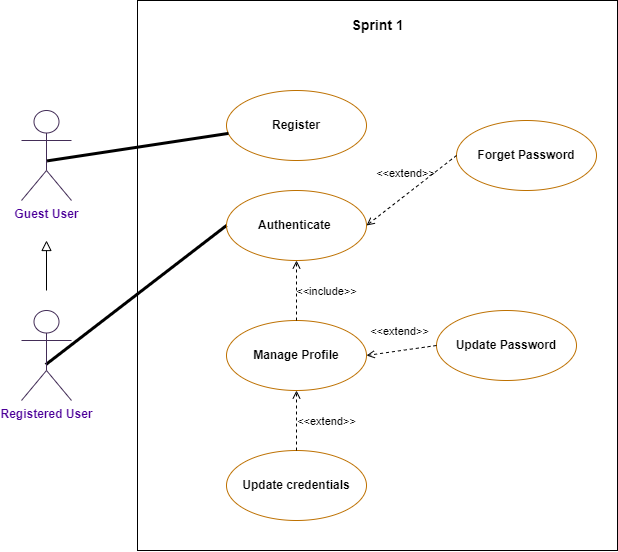
\includegraphics[height=12cm]{images/chap2/Sprint1UC.png}
    \caption{Sprint 1 use case diagram}
    \label{fig:enter-label}
\end{figure}


\section{User story n°1 : Configurable application}
Since this application is meant to be purchased by many clients , we provided the luxury of customization and to grant for every client the possibility of having an application that meets his needs .
This is done thanks to the services that import the clients on starting the application ,this process can be better described with the next illustration :

\begin{figure}[H] 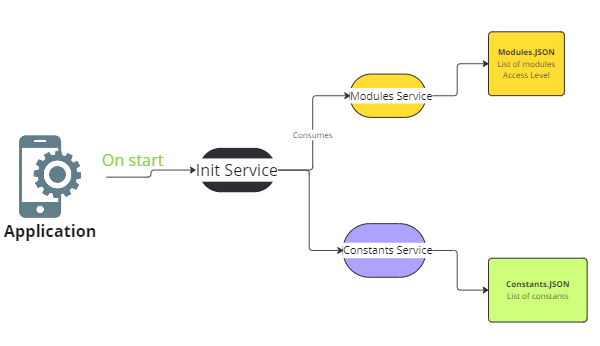
\includegraphics[width=0.90\textwidth]{images/chap2/config.png}
    \caption{Configurable Application illustration}
    \label{fig:enter-label}
\end{figure}

This approach is based on consuming raw values from JSON files that the application's owner can edit manually or via an interface in our case we split the load of data on specific services to ensure the ease of use  and the possibility for scaling 



\section{User story n°2 : Navigation}
As the global use case diagram shows that the application has some modules that require authentication whereas others don't ,so we developed a mechanism to attend this behavior , the following flowchart explain it well
\begin{figure}[H] 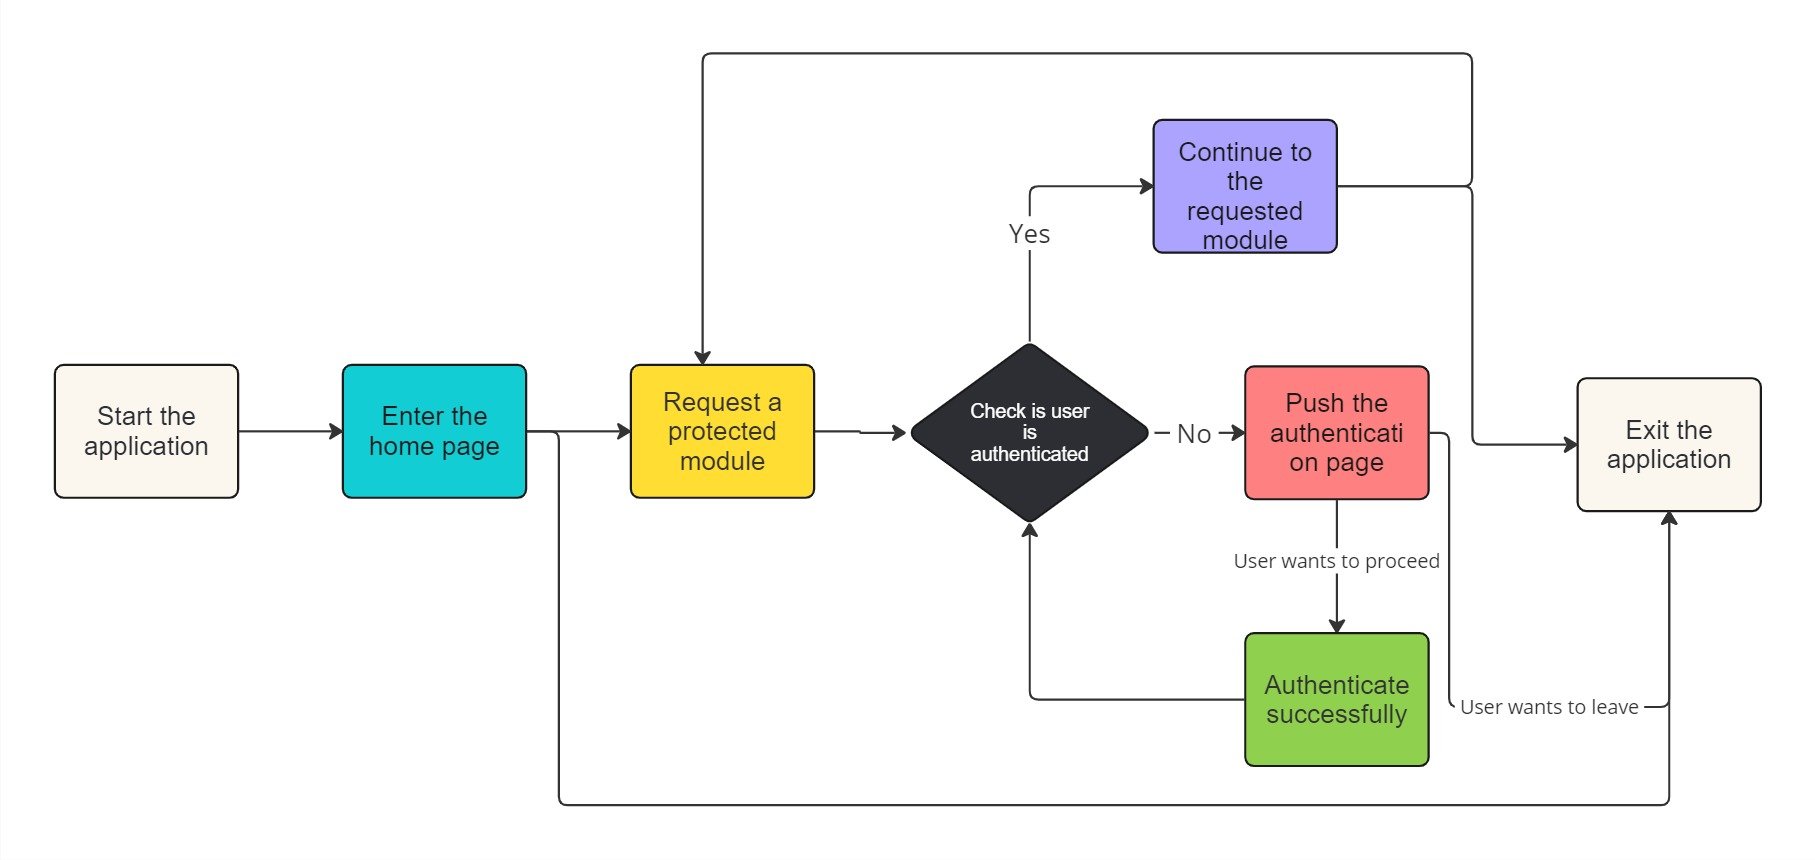
\includegraphics[height=8cm]{images/chap2/Pmdl.jpg}
    \caption{Module protection flowchart}
    \label{fig:enter-label}
\end{figure}
\newpage
\subsection{Realization}
The navigation system is split to two main parts: module navigator with bottom tabs and the application management with the drawer navigator
\begin{figure}[H]
\begin{minipage}{0.3\textwidth}
    \centering
    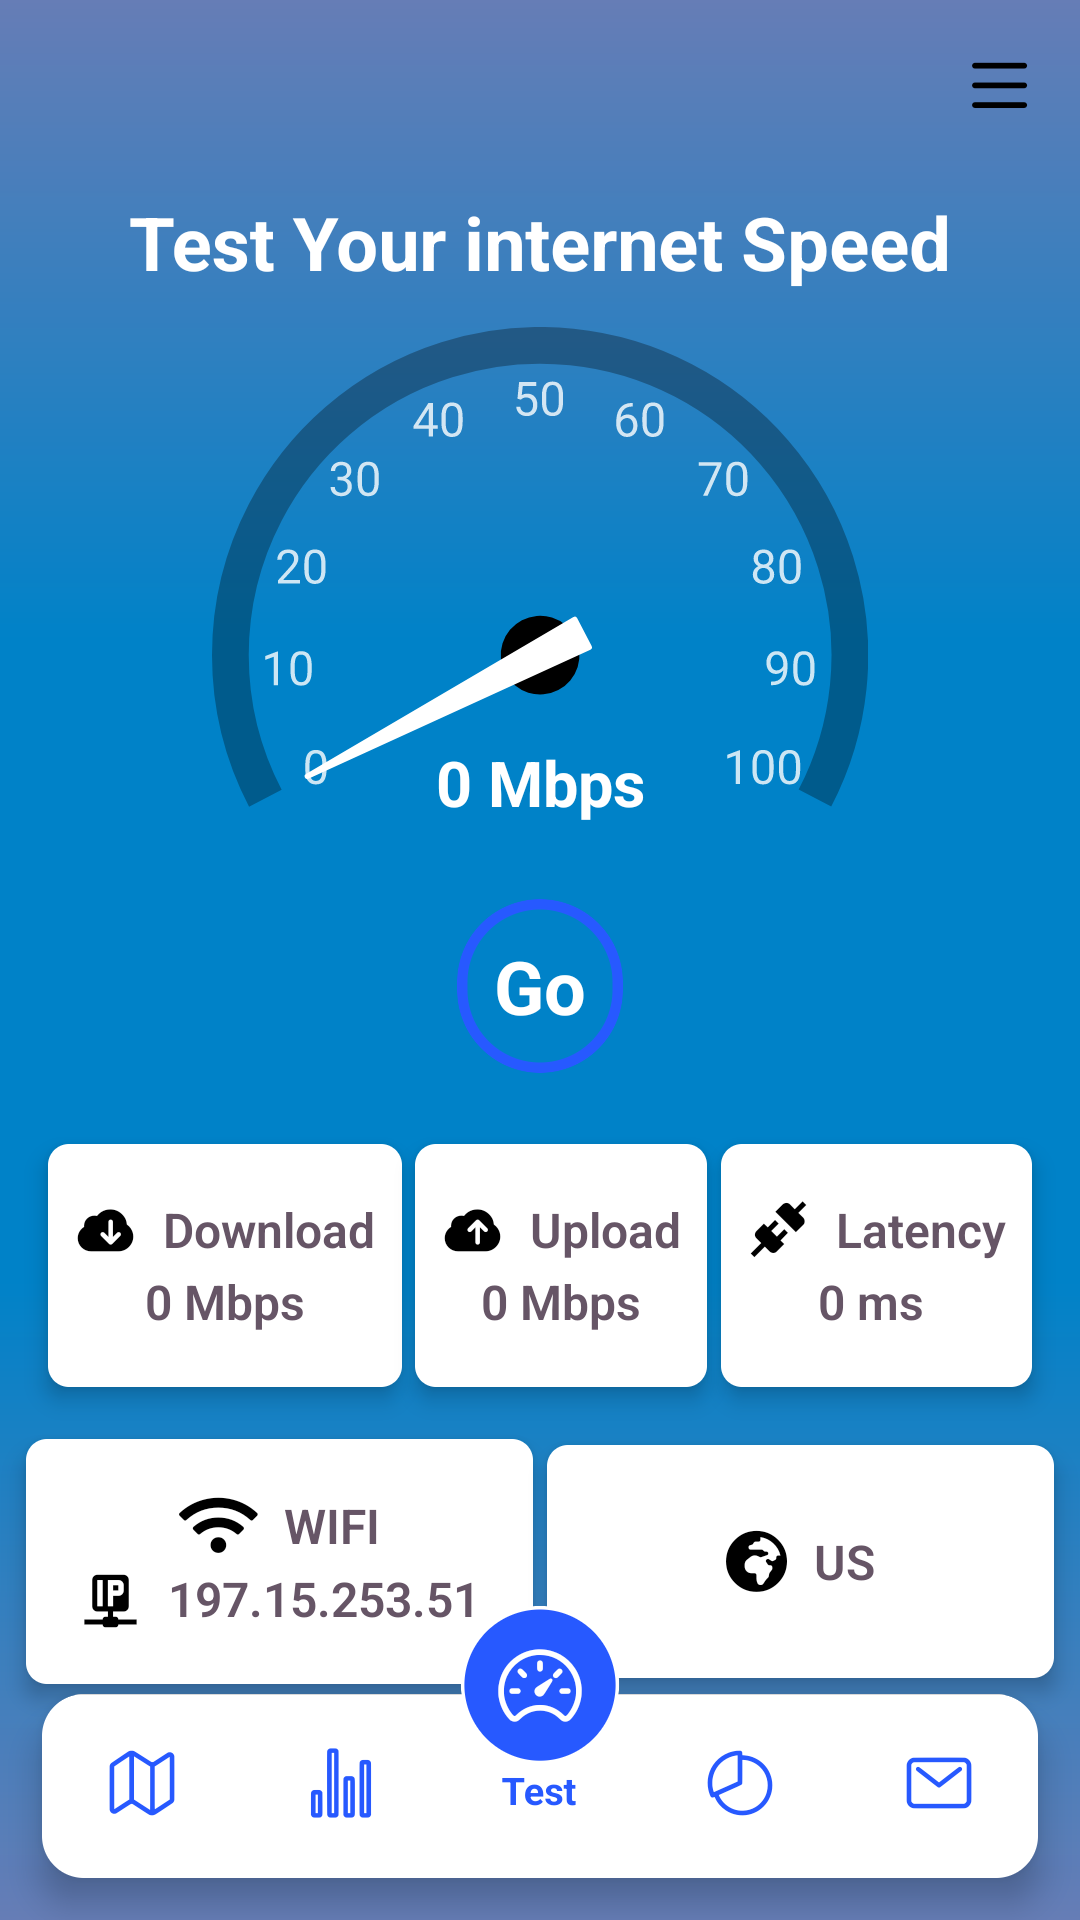
\includegraphics[width=\linewidth]{images/chap2/nav1.png}
    % \caption{Forget Password Sequence Diagram Part 1}
    \label{fig:login-form}
\end{minipage}\hfill
\begin{minipage}{0.3\textwidth}
    \centering
    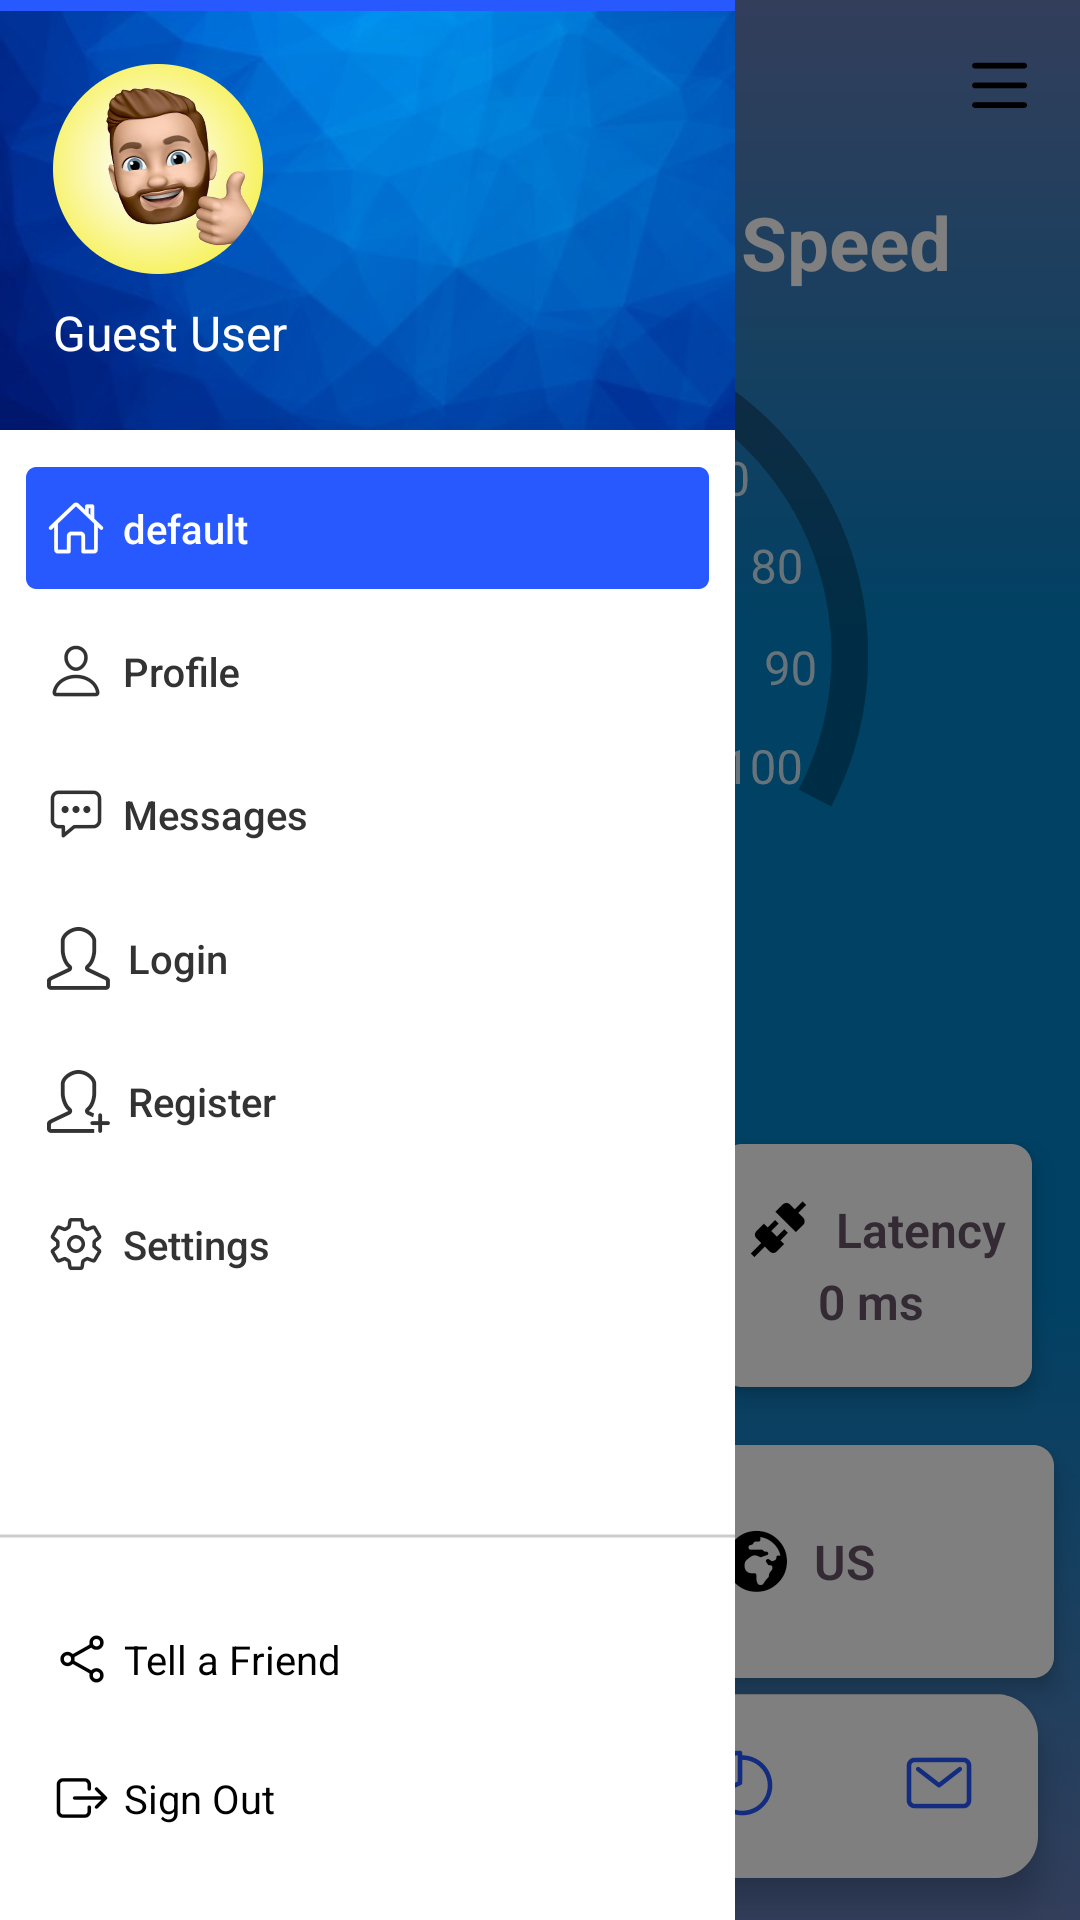
\includegraphics[width=\linewidth]{images/chap2/nav2.png}
    \label{fig:login-form-filled}
\end{minipage}
    \caption{Navigation system}
\end{figure}
\newpage
\section{User story n°3 : Authentication}
\subsection*{\textbf{\underline{Text description of the "Register" use case}}}
In the table below , we will have a clear idea about the  Register use case : 
\begin{table}[H]
    % \centering
    \renewcommand{\arraystretch}{1.5}  
   \begin{tabular}{|p{0.25\textwidth}|p{0.75\textwidth}|}
   \hline
        \textbf{Use Case} &  Register  \\   \hline
        
        \textbf{Actor(s) } & Guest User  \\   \hline
        \textbf{Pre-condition} &     
             The user requested the registration page
\\   \hline
        \textbf{Post-condition} & User will be redirected to the home page  \\  \hline

                \textbf{Principal scenario} & 
                \begin{enumerate}[left=0pt]
                \item The user requests the register screen .
                \item The system displays the registration page.
                \item The user enters his information.
                \item The user submits his information.
                \item The system validates the users information.
                \item The user is redirected to the home page.
                \end{enumerate}  \\   \hline
                 
          \textbf{Alternative\newline scenario} & 
      
             
             If the account  already exist , an error  message will appear to the user .\newline
            If an error related to the data occurs, a proper message will appear to the user to check his input.
 \\   \hline
\end{tabular}
  
         \caption{Text description of the “ Register” use case}
    \label{tab:my_label}
\end{table}

\newpage
\subsection*{\textbf{\underline{Text description of the "Login" use case}}}

\vspace{0.25cm}
In the table below , we will have a clear idea about the Login use case : 

\begin{table}[H]
    % \centering
    \renewcommand{\arraystretch}{1.5}
    
   \begin{tabular}{|p{0.25\textwidth}|p{0.7\textwidth}|}
   \hline
     
        \textbf{Use Case} & Login  \\   \hline
        
        \textbf{Actor(s) } & Registered User  \\   \hline
        \textbf{Pre-condition} &  
        \begin{itemize}[left=0pt]
             \renewcommand\labelitemi{\textbf{\Huge .}}
             
            \item The account has to be already created.
            \item The user requested the login page .
        \end{itemize} \\   \hline
        \textbf{Post-condition} & The use redirected to the previous page  \\  \hline
                \textbf{Principal scenario} & 
                \begin{enumerate}[left=0pt]
                \item The user requests the login screen .
                \item The system displays the login page.
                \item The user enter his information.
                \item The user submits his information.
                \item The system validates the users information.
                \item The user is redirected to the Test page.
                \end{enumerate}  \\   \hline                 
          \textbf{Alternative\newline scenario} & 
        \begin{itemize}[left=0pt]
             \renewcommand\labelitemi{\textbf{\Huge .}}
            \item If the account  does not exist , an error  message will appear to the user .
            \item If an error related to the data occurs , a proper message will appear to the user to check his input.
        \end{itemize} \\   \hline

\end{tabular}  
         \caption{Text description of the “Login” use case}
    \label{tab:my_label}
\end{table}

\subsection*{\textbf{\underline{Text description of the "Forget Password " use case}}}

\vspace{0.25cm}
In the table below , we will have break down the Forget Password use case : 

\begin{table}[H]
    % \centering
    \renewcommand{\arraystretch}{1.5}
    
   \begin{tabular}{|p{0.25\textwidth}|p{0.7\textwidth}|}
   \hline
     
        \textbf{Use Case} &Forget password  \\   \hline
        
        \textbf{Actor(s) } & Registered user  \\   \hline
        \textbf{Pre-condition} &  
        \begin{itemize}[left=0pt]
             \renewcommand\labelitemi{\textbf{\Huge .}}
            \item The account has to be already created
        \end{itemize} \\   \hline


        \textbf{Post-condition} & User's password is updated \\  \hline

                \textbf{Principal scenario} & 
                \begin{enumerate}[left=0pt]
                \item The user enter his email  .
                \item The system sends a verification mail that contains a secret code, to the provided email by the user  .
                \item The user submits the code .
                \item The system checks the code .
                \item The system displays a reset password form.
                \item The user fill the form with password and confirm password
                \item The system updates the database.
                \item A success message is displayed and the user is asked to login.
                \end{enumerate}  \\   \hline
                 
          \textbf{Alternative\newline scenario} & 
        \begin{itemize}[left=0pt]
             \renewcommand\labelitemi{\textbf{\Huge .}}
            \item If the account does not exist a warning message appears .
            \item If code is wrong a warning message appears and the user can ask for an other verification code.
            \item If the input is wrong the user is asked to check again.
            \item If the password is the same as the already saved in the database the user get warned.
        \end{itemize} \\   \hline
\end{tabular}
  
         \caption{Text description of the “Forget Password” use case}
    \label{tab:my_label}
\end{table}
% To realisation section
% 
% 

% Class diagram

% ###########################
% Sequence Diag
% 
% 
% ###########################
\subsection{Sequence Diagrams}
\subsubsection{Register Sequence Diagram}
\begin{figure}[H]
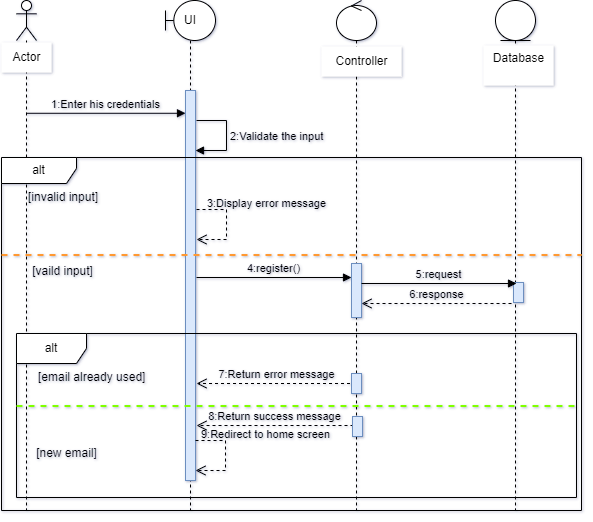
\includegraphics[width=0.98\textwidth]{images/chap2/registerSeq_c.png}
    \caption{“Register” Sequence Diagram}
    \label{fig:enter-label}    
\end{figure}
% ###########################
\subsubsection{Login Sequence Diagram}
\begin{figure}[H]
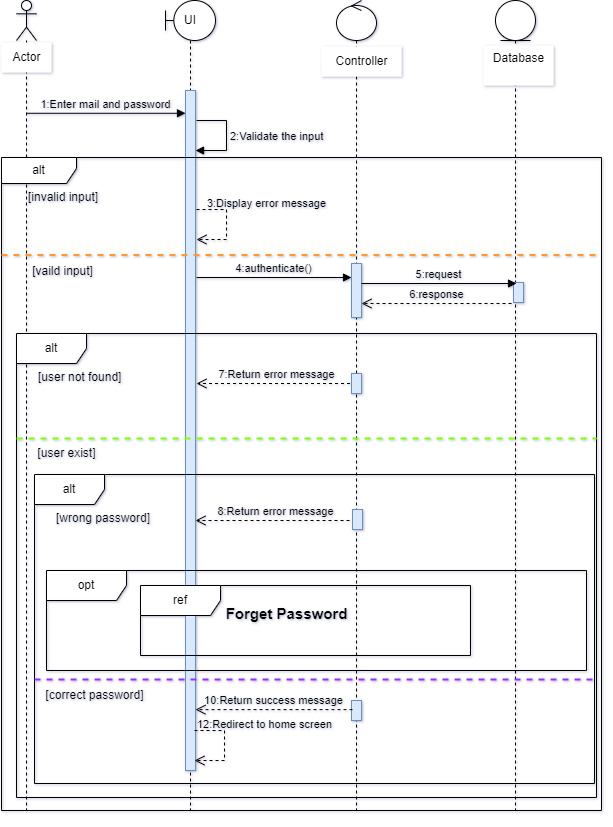
\includegraphics[width=0.98\textwidth]{images/chap2/AuthSeq_c.png}
    \caption{“Login” Sequence Diagram}
    \label{fig:enter-label}
\end{figure}

% ###########################
\subsubsection{Forget password  Sequence Diagram}
\begin{figure}[H]
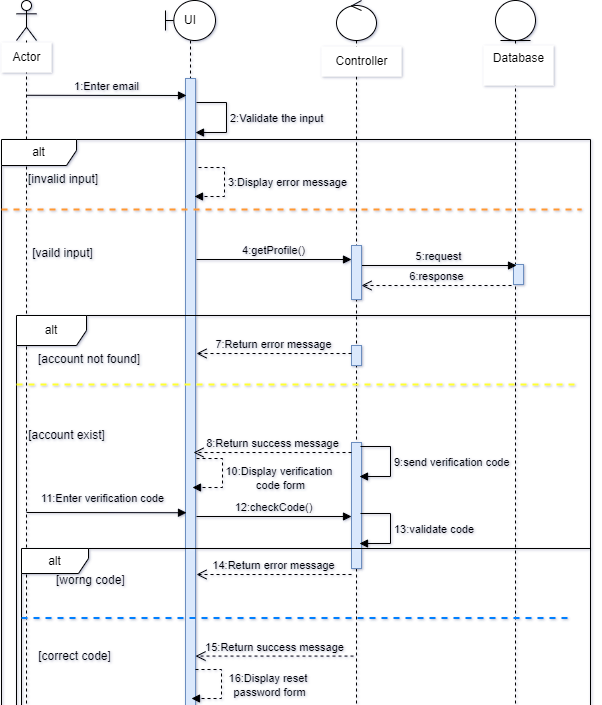
\includegraphics[width=0.98\textwidth]{images/chap2/resetPassword_cp1.png}
    % \caption{“Forget Password” Sequence Diagram}
    \label{fig:enter-label}    
\end{figure}
\begin{figure}[H]
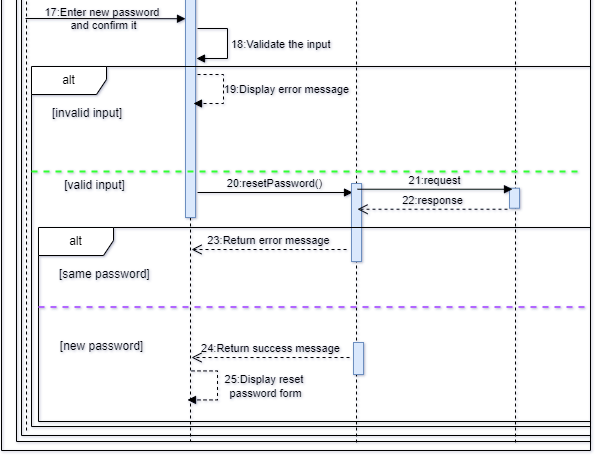
\includegraphics[width=0.98\textwidth]{images/chap2/resetPassword_cp2.png}
    \caption{“Forget Password” Sequence Diagram}
    \label{fig:enter-label}    
\end{figure}
% ###########################
\subsection{Class diagram }
Here is the class diagram that describes User entity in our database
\begin{figure}[H]
\begin{center}
    
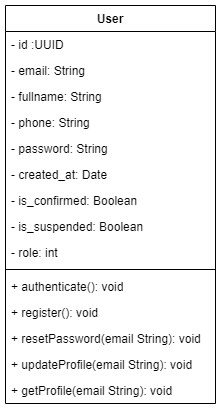
\includegraphics[width=0.3\textwidth]{images/chap2/userClass.png}
    \caption{Class diagram}
    \label{fig:enter-label} 
\end{center}
\end{figure}
% 
% 
% 
\subsection{Realization}
\subsubsection{Access Token and Refresh Token mechanism}
The authentication state of a user is generally represented by a token that is stored in some secured place in the application,this is the convention often used in the software industry ,in this application we used the JWT tokens to hold the user's authentication state .
For better securing our application we implemented a common mechanism of access/refresh token that's described by the figure below :
\begin{figure}[H]
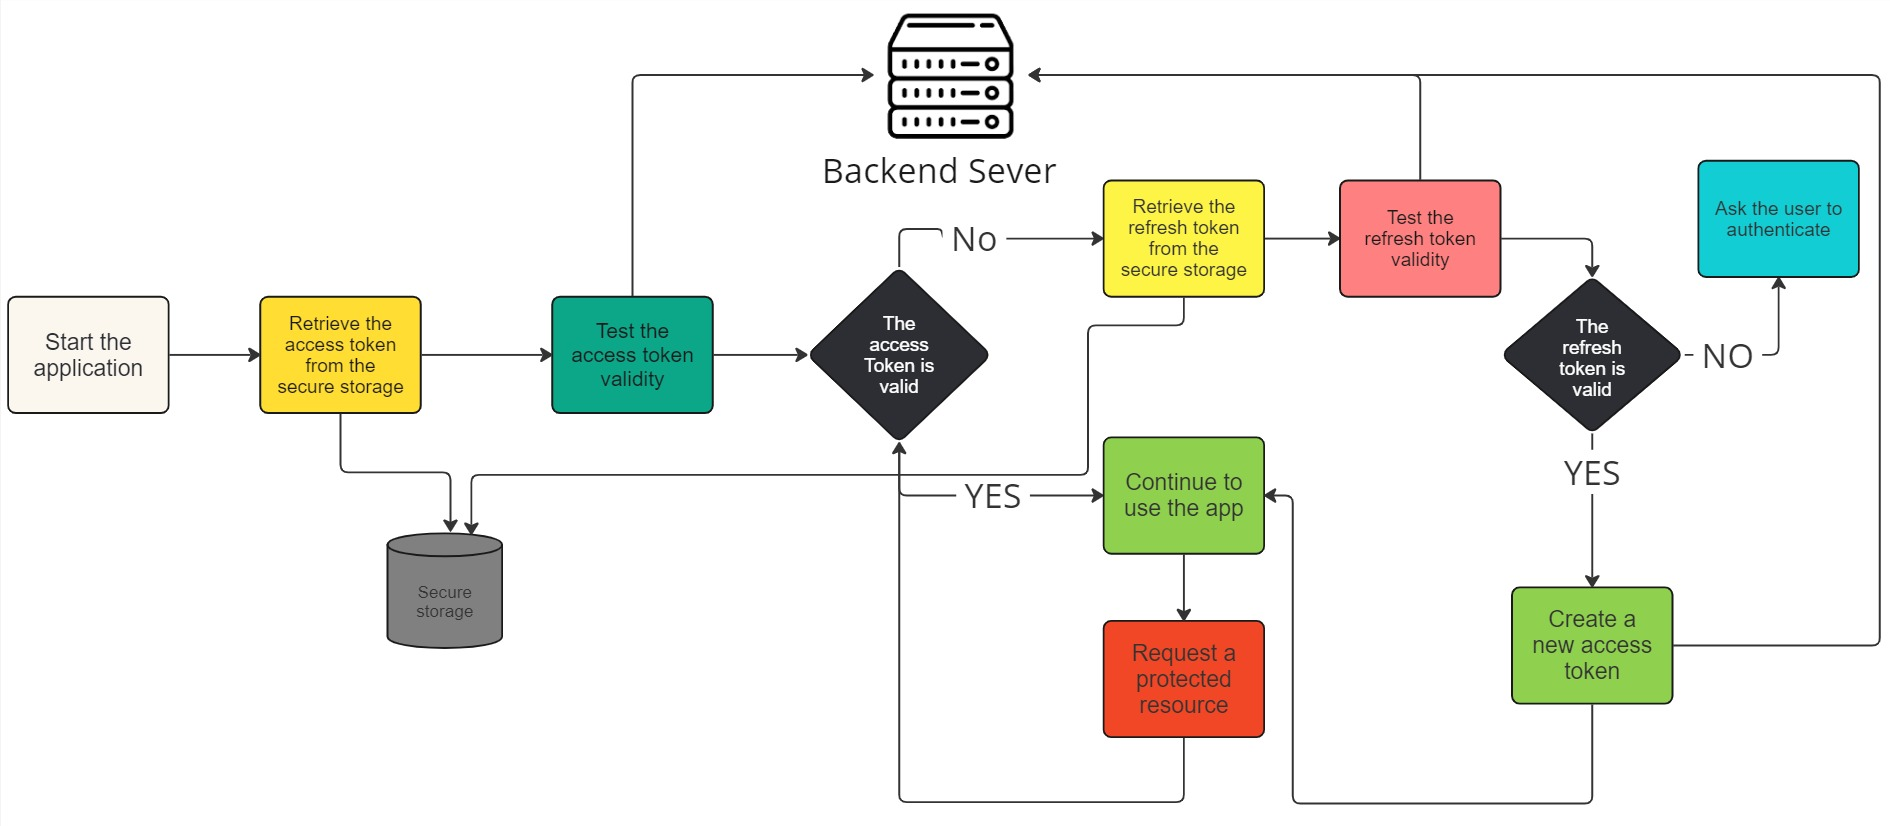
\includegraphics[width=1\textwidth]{images/chap2/refTkn.jpg}
    \caption{Access token and refresh token mechanism}
    \label{fig:enter-label}
\end{figure}
\subsubsection{Registration}
This is the interface that the user can create within 
\begin{figure}[H]
\begin{minipage}{0.45\textwidth}
    \centering
    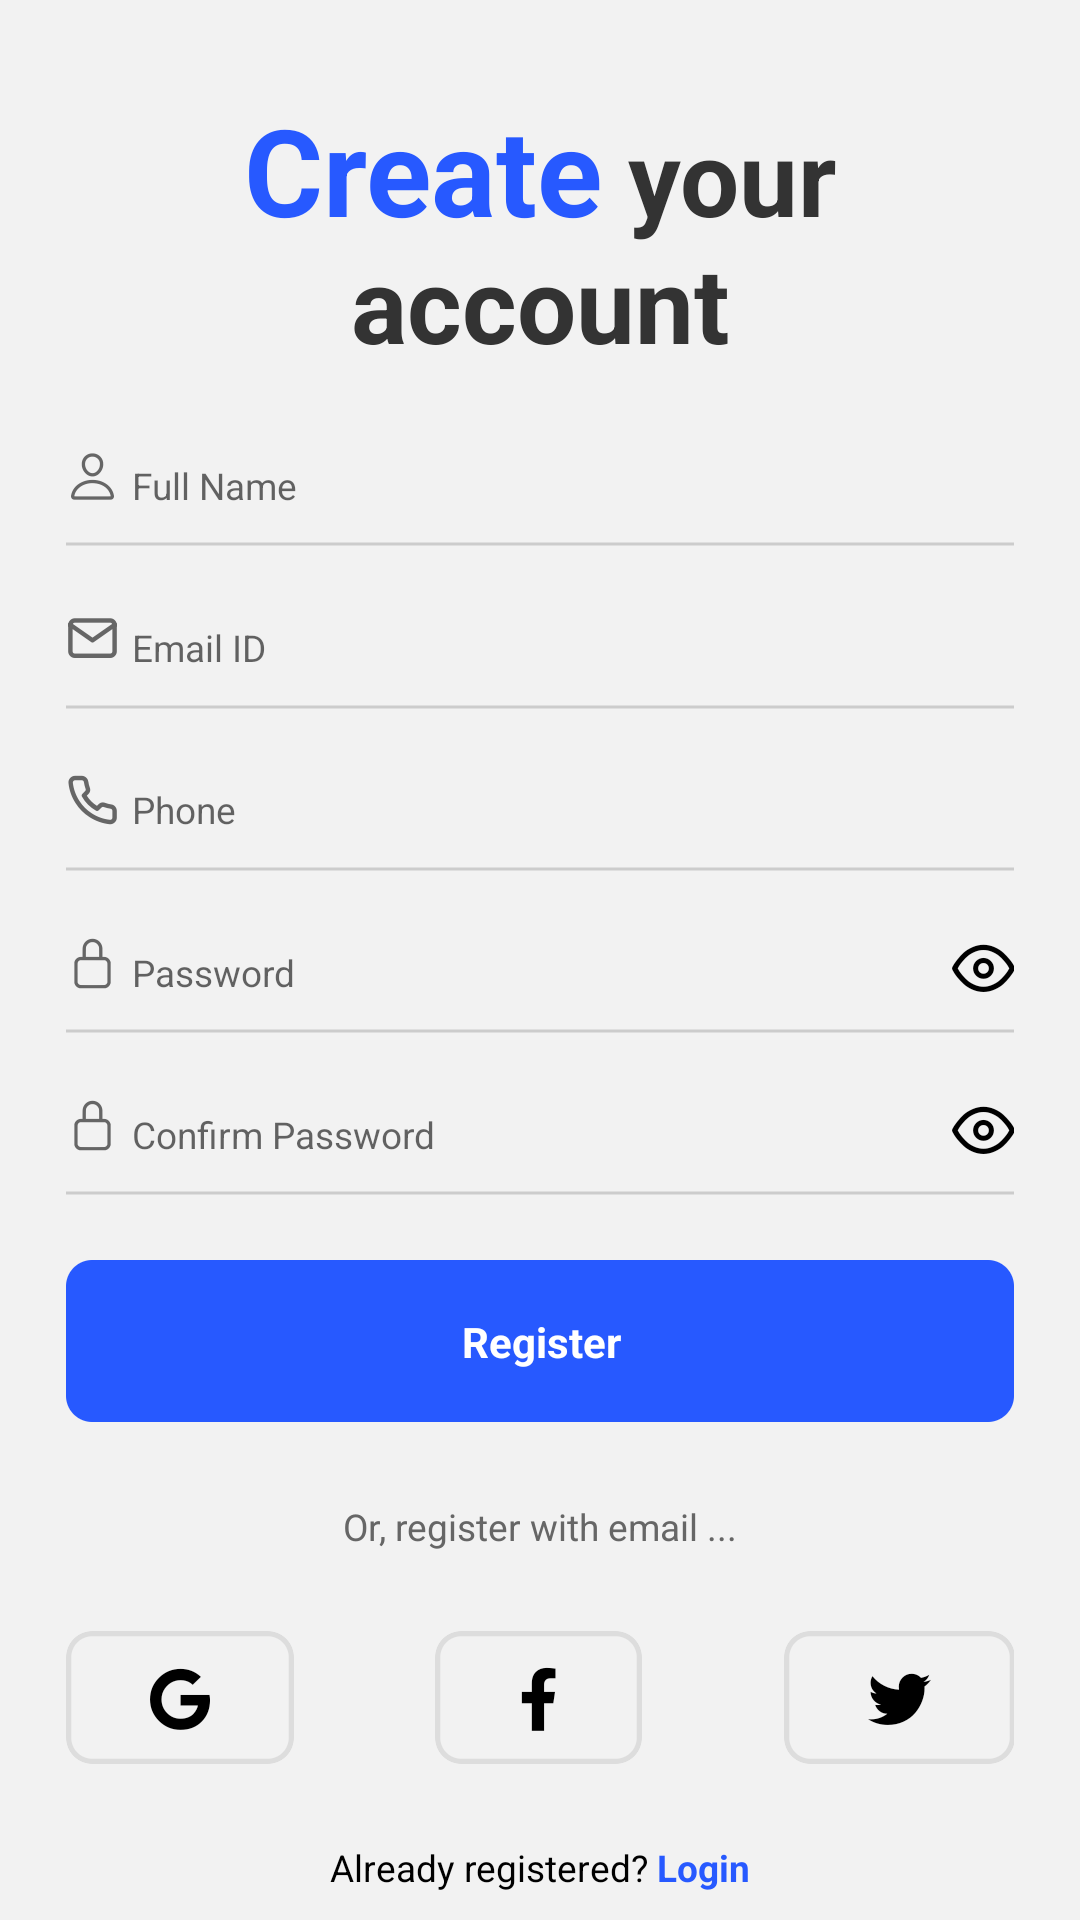
\includegraphics[width=\linewidth]{images/chap2/RegisterForm.png}
    \label{fig:login-form}
\end{minipage}\hfill
\begin{minipage}{0.45\textwidth}
    \centering
    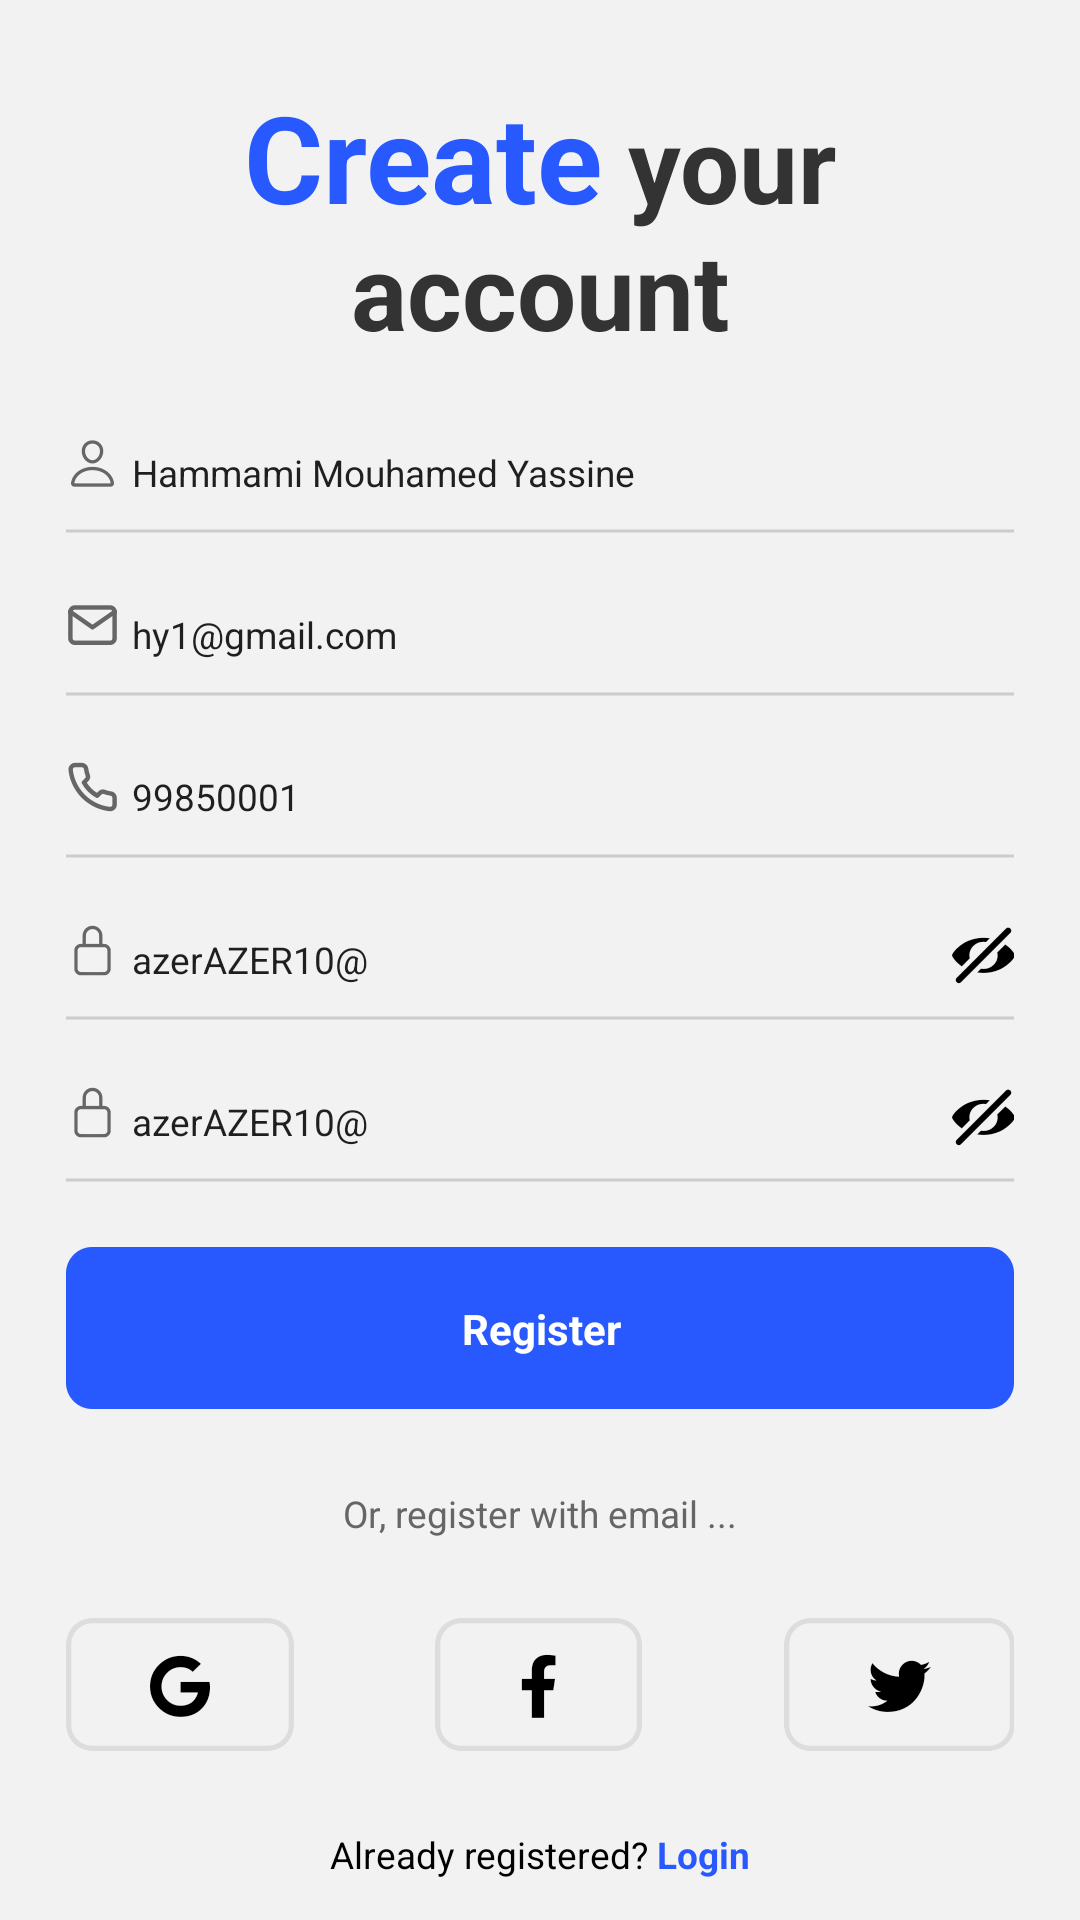
\includegraphics[width=\linewidth]{images/chap2/RegisterFormFilled.png}
    % \caption{Forget Password Sequence Diagram Part 2}
    \label{fig:login-form-filled}
\end{minipage}
    \caption{Registration user interface}
\end{figure}
% ###############
\newpage
\subsubsection{Authentication}
Via this interface the user can enter his credentials and authenticate to the application 
\begin{figure}[H]
\begin{minipage}{0.45\textwidth}
    \centering
    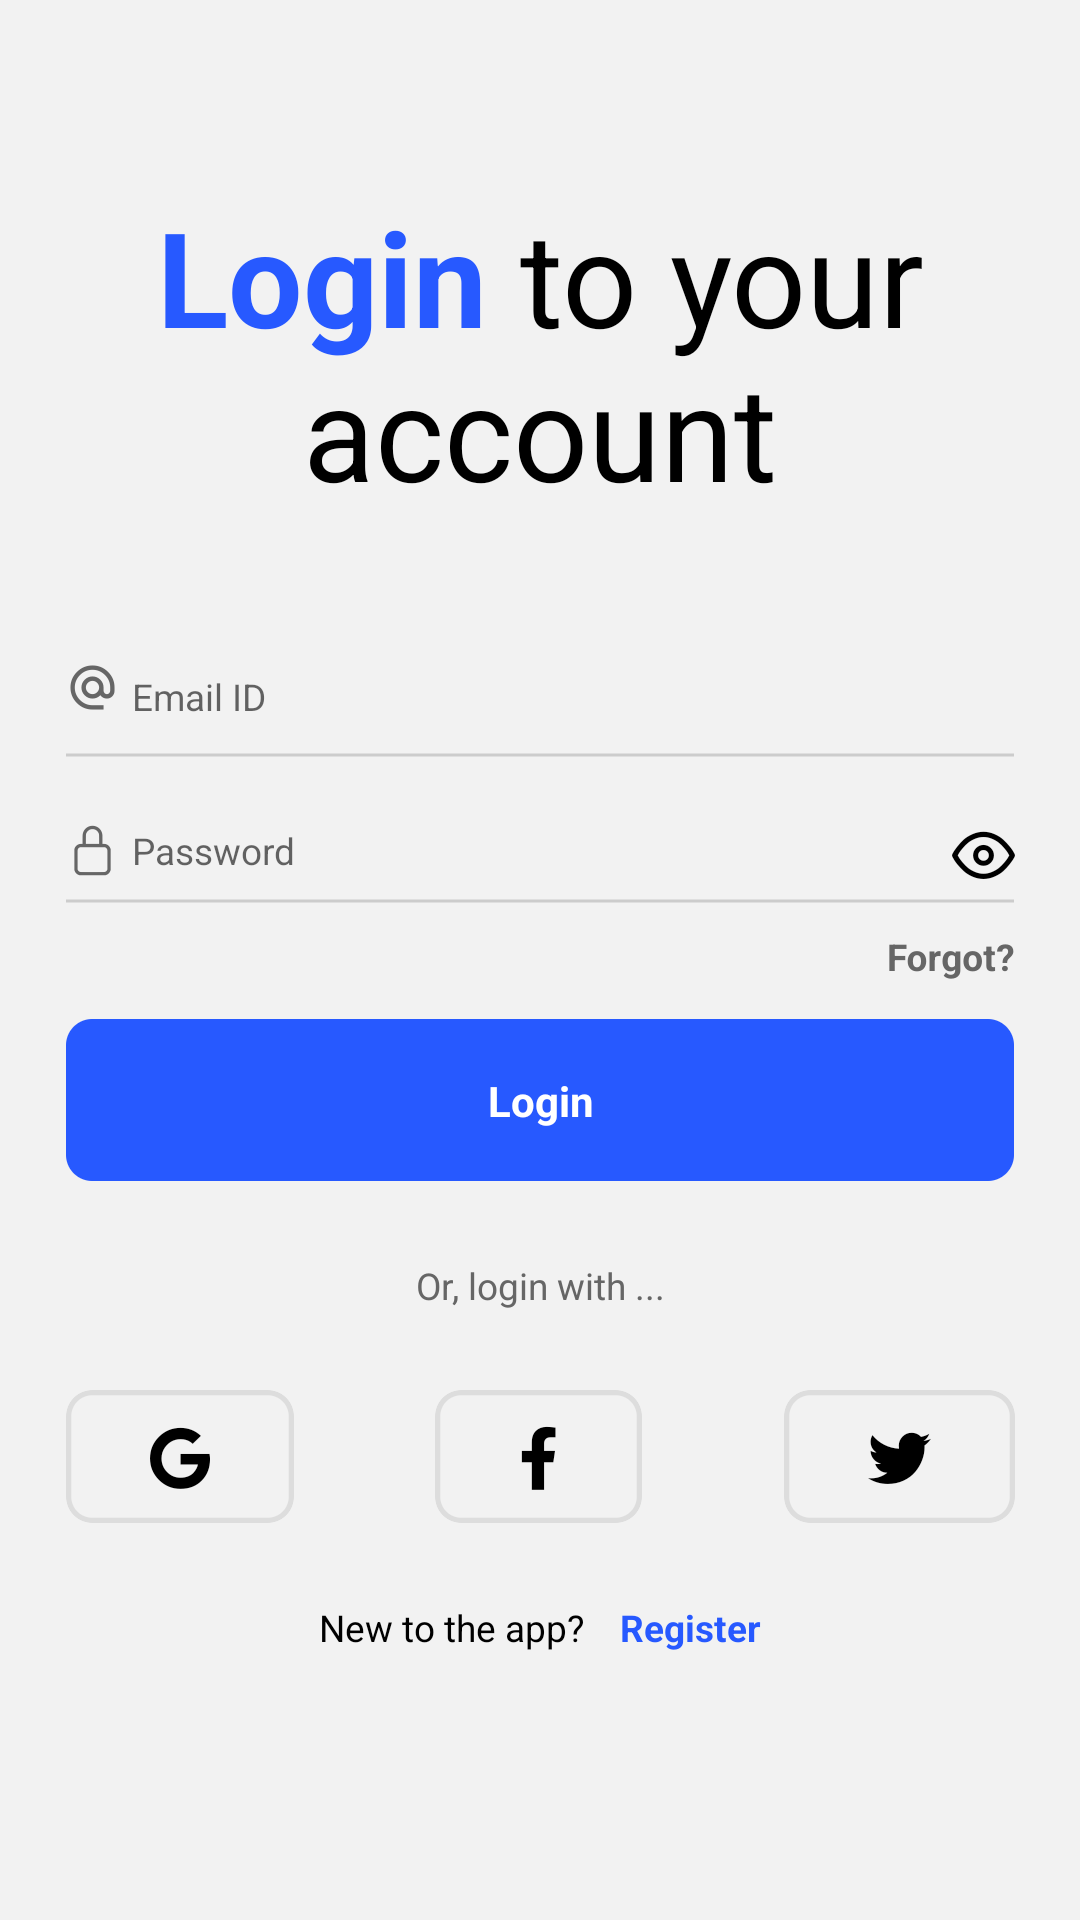
\includegraphics[width=\linewidth]{images/chap2/LoginForm.png}
    % \caption{Forget Password Sequence Diagram Part 1}
    \label{fig:login-form}
\end{minipage}\hfill
\begin{minipage}{0.45\textwidth}
    \centering
    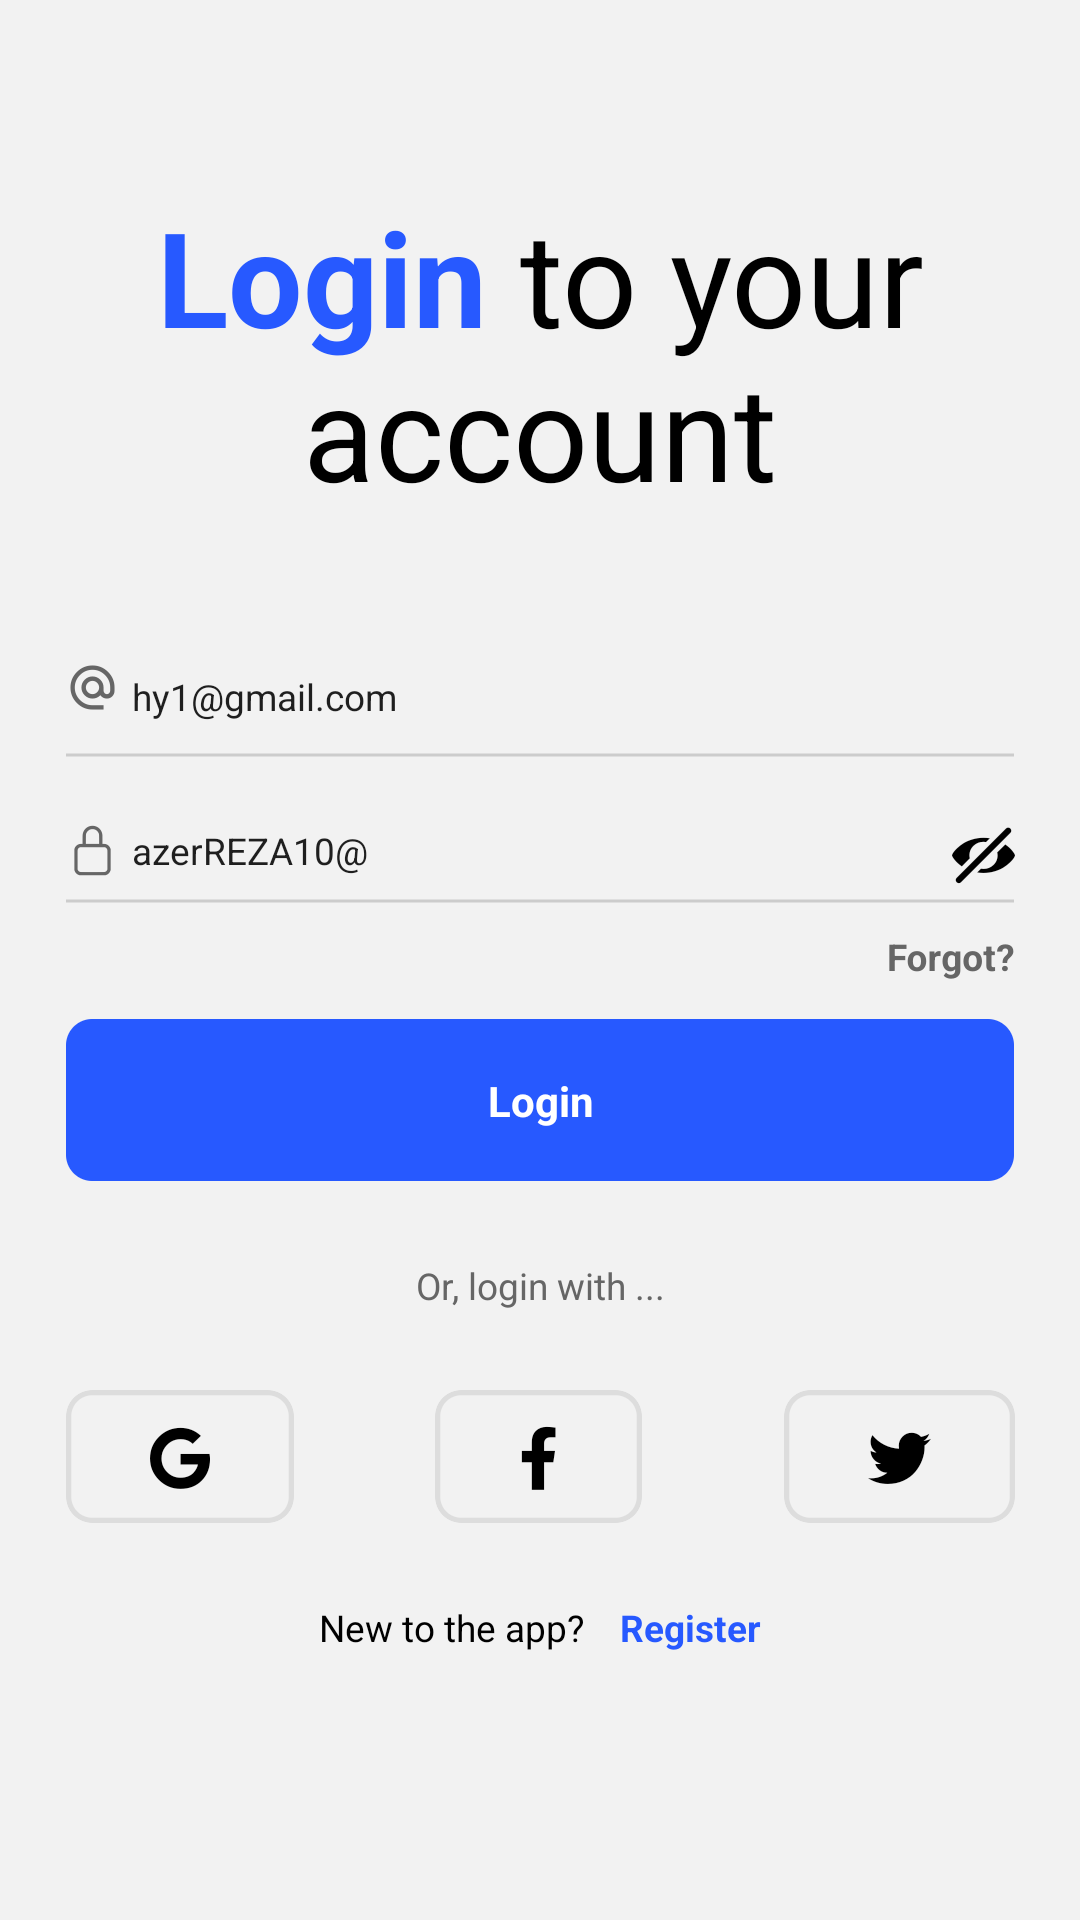
\includegraphics[width=\linewidth]{images/chap2/LoginFormFilled.png}
    \label{fig:login-form-filled}
\end{minipage}
    \caption{Login user interface}
\end{figure}
% ###########################
\newpage
\section{User story n°4 : Profile management}
\subsection*{\textbf{\underline{Text description of the "Update Credentials" use case}}}

\vspace{0.25cm}
In the table below , we will explain the Update Credentials use case : 

\begin{table}[H]
    % \centering
    \renewcommand{\arraystretch}{1.5}
    
   \begin{tabular}{|p{0.25\textwidth}|p{0.68\textwidth}|}
   \hline
     
        \textbf{Use Case} &Update Credentials  \\   \hline
        
        \textbf{Actor(s) } & Registered User  \\   \hline
        \textbf{Pre-condition} &  
        \begin{itemize}[left=0pt]
             \renewcommand\labelitemi{\textbf{\Huge .}}
            \item The user has to be authenticated 
            \item The user request the profile page 
        \end{itemize} \\   \hline


        \textbf{Post-condition} & User's profile is updated \\  \hline

                \textbf{Principal scenario} & 
                \begin{enumerate}[left=0pt]
                \item The user requests the profile page
                \item The system displays the profile page
                \item The user enters his new credentials
                \item The user confirms the modification
                \item The system updates the user credentials .
                \item The system displays the new credentials .
                \end{enumerate}  \\   \hline
                 
          \textbf{Alternative\newline scenario} & 
        \begin{itemize}[left=0pt]
             \renewcommand\labelitemi{\textbf{\Huge .}}
            \item If the input is wrong a warning message appears .

        \end{itemize} \\   \hline
\end{tabular}
         \caption{Text description of the “Update Credentials” use case}
    \label{tab:my_label}
\end{table}

\newpage
\subsection*{\textbf{\underline{Text description of the "Update Password" use case}}}

\vspace{0.25cm}
In the table below , we will explain the Update Password use case : 

\begin{table}[H]
    % \centering
    \renewcommand{\arraystretch}{1.5}
    
   \begin{tabular}{|p{0.25\textwidth}|p{0.68\textwidth}|}
   \hline
     
        \textbf{Use Case} &Update Password  \\   \hline
        
        \textbf{Actor(s) } & Registered User  \\   \hline
        \textbf{Pre-condition} &  
        \begin{itemize}[left=0pt]
             \renewcommand\labelitemi{\textbf{\Huge .}}
            \item The user has to be authenticated 
            \item The user request the profile page 
        \end{itemize} \\   \hline


        \textbf{Post-condition} & User's password is updated \\  \hline

                \textbf{Principal scenario} & 
                \begin{enumerate}[left=0pt]
                \item The user requests the profile screen
                \item The user requests the change password screen
                \item The system displays the change password screen
                \item The user enters his new password and confirm it 
                \item The user confirms the modification
                \item The system updates the user's password
                \end{enumerate}  \\   \hline
                 
          \textbf{Alternative\newline scenario} & 
        \begin{itemize}[left=0pt]
             \renewcommand\labelitemi{\textbf{\Huge .}}
            \item If the input is wrong a warning message appears .
            \item If the password is similar to the old one, a failure message appears.
        \end{itemize} \\   \hline
\end{tabular}
         \caption{Text description of the “Update Password” use case}
    \label{tab:my_label}
\end{table}
\subsection{Sequence diagram}
\begin{figure}[H]
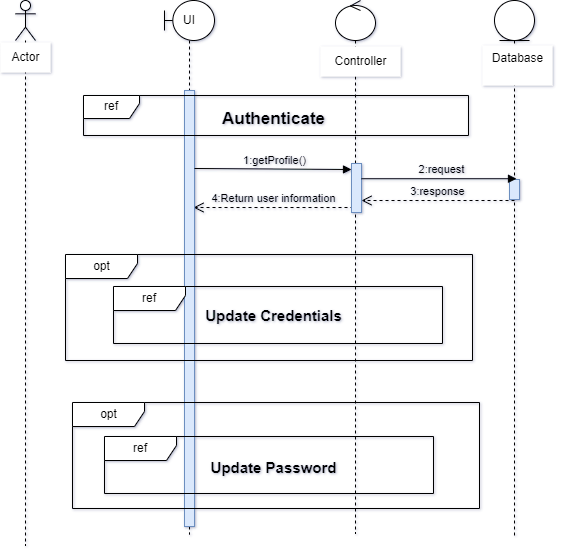
\includegraphics[width=0.98\textwidth]{images/chap2/manageProfile_c.png}
    \caption{“Manage Profile” sequence Diagram}
    \label{fig:enter-label}    
\end{figure}
\begin{figure}[H]
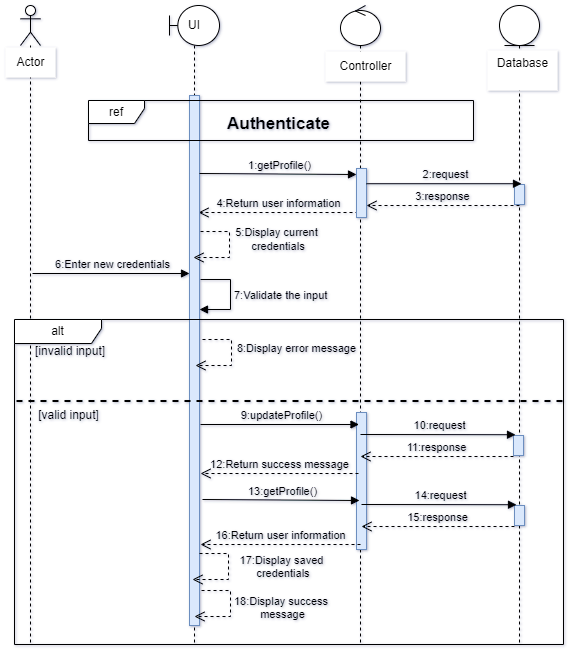
\includegraphics[width=0.98\textwidth]{images/chap2/updateCred.png}
    \caption{“Update Credentials” sequence Diagram}
    \label{fig:enter-label}    
\end{figure}
\begin{figure}[H]
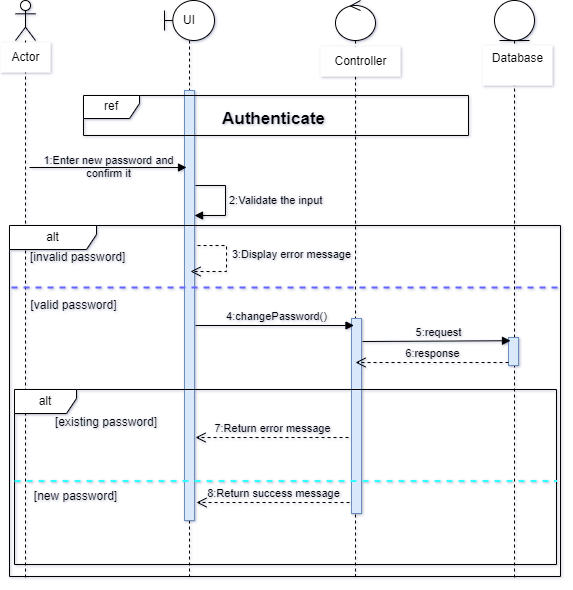
\includegraphics[width=0.98\textwidth]{images/chap2/changePassword_c.png}
    \caption{“Update Password” sequence Diagram}
    \label{fig:enter-label}    
\end{figure}
% 
% 
% 
\newpage
\subsection{Realization}
% ###############
\subsubsection{Manage Profile interfaces}
Via this interface the user can update information related to his profile like credentials and password
\begin{figure}[H]
\begin{minipage}{0.45\textwidth}
    \centering
    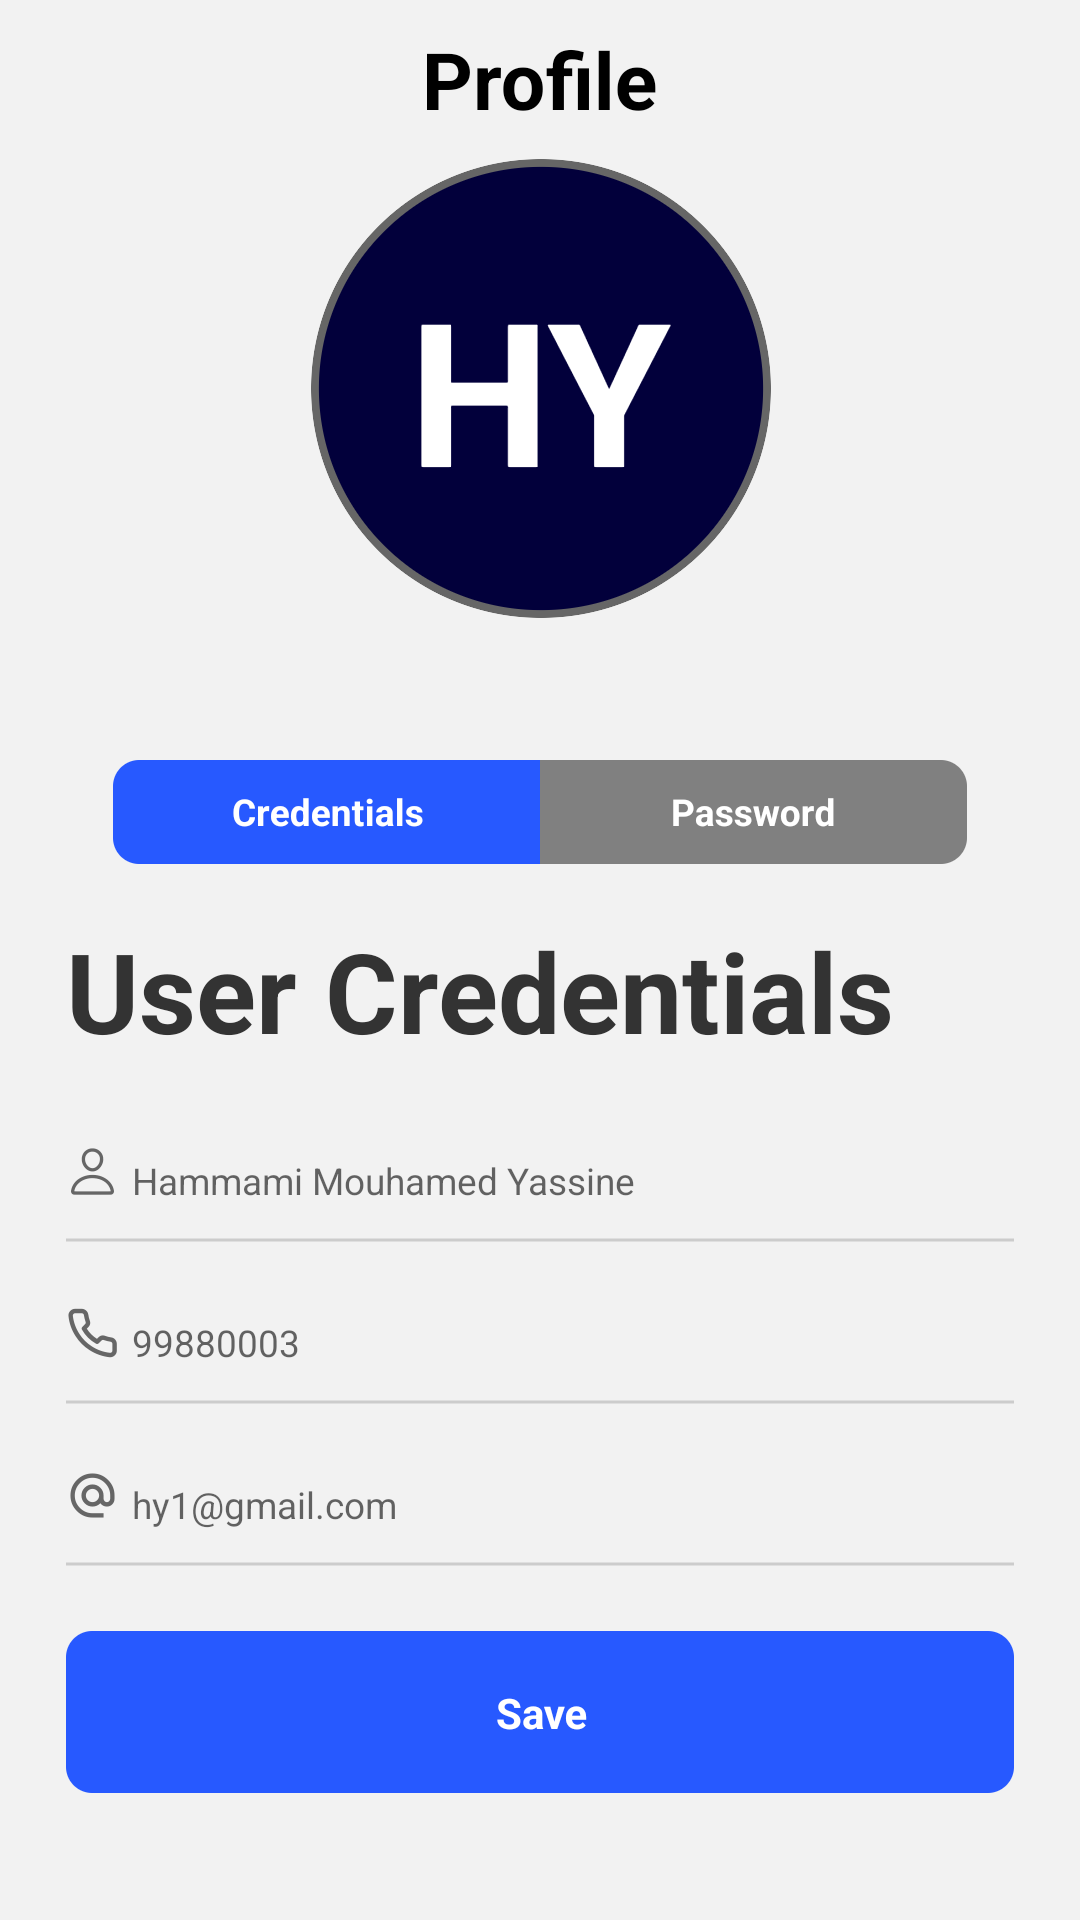
\includegraphics[width=\linewidth]{images/chap2/editUserCred.png}
    % \caption{Forget Password Sequence Diagram Part 1}
    \label{fig:login-form}
\end{minipage}\hfill
\begin{minipage}{0.45\textwidth}
    \centering
    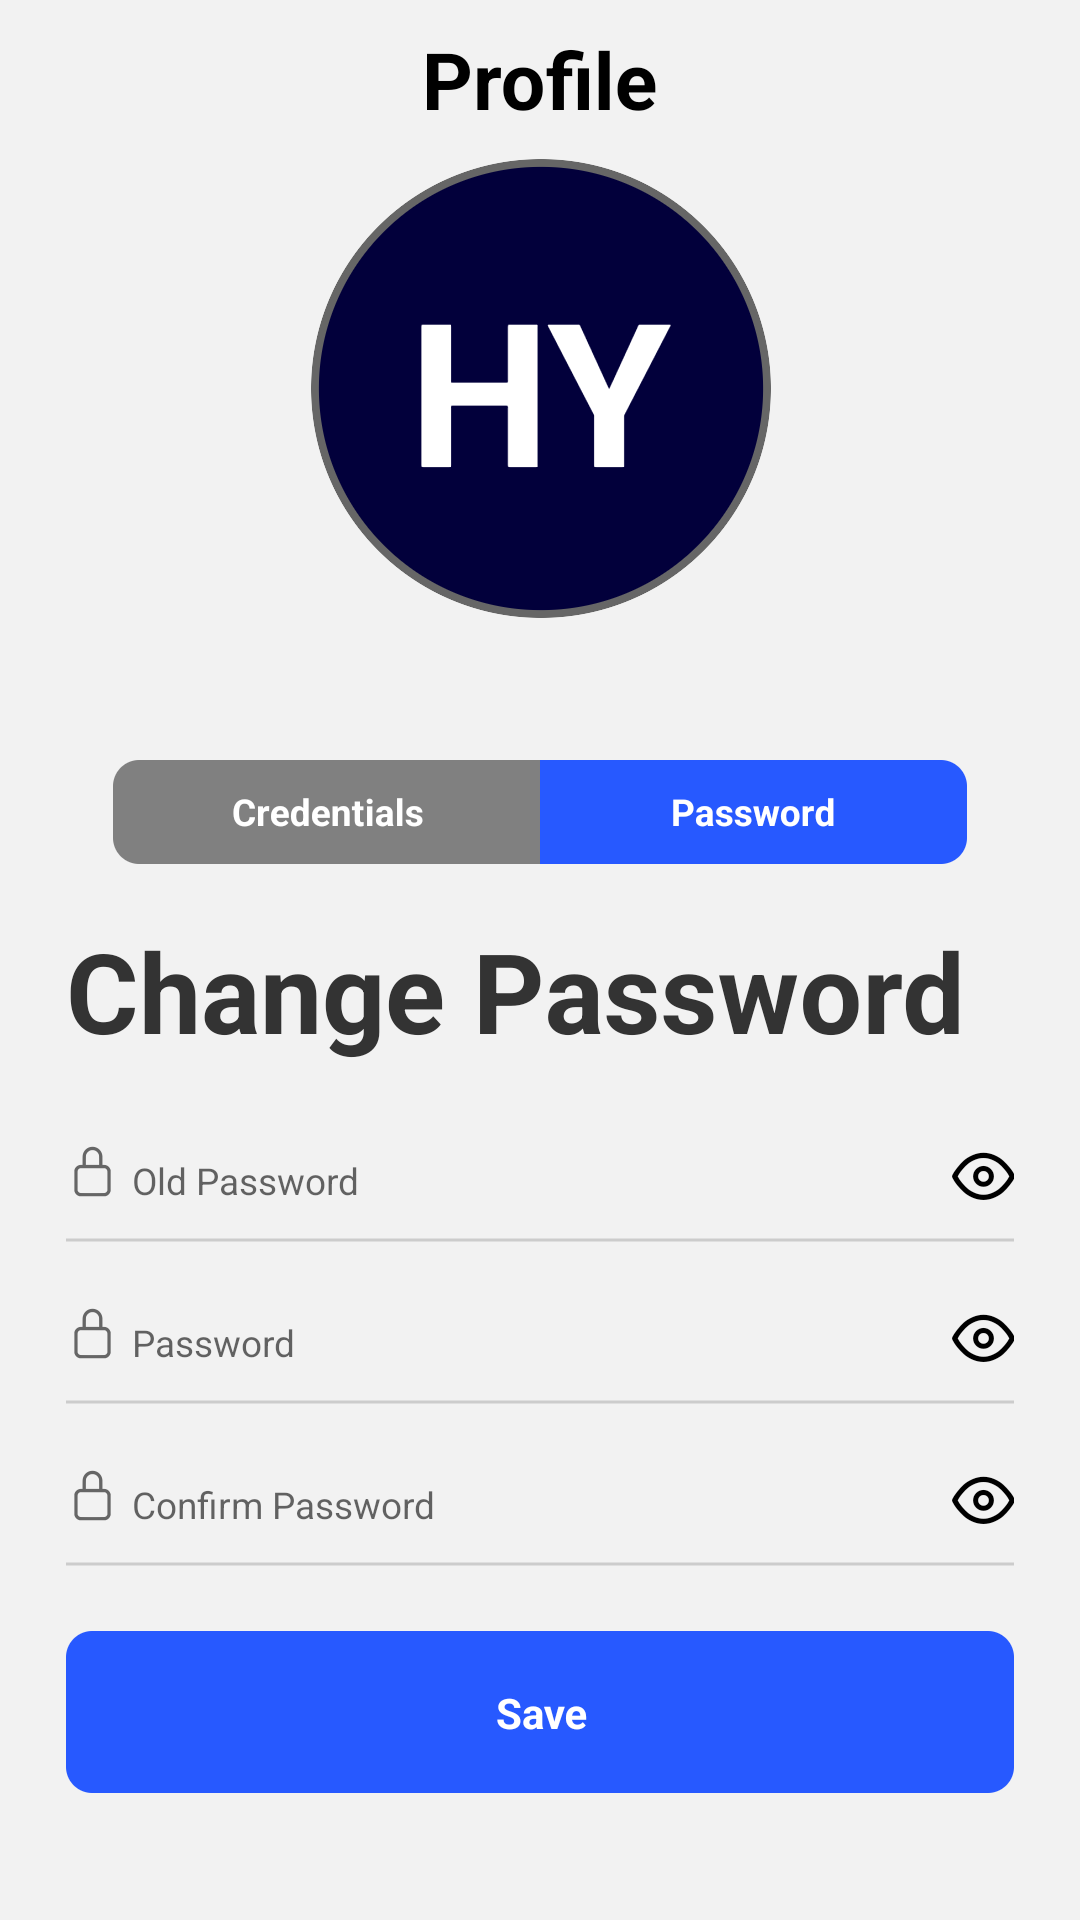
\includegraphics[width=\linewidth]{images/chap2/editPwd.png}
    \label{fig:login-form-filled}
\end{minipage}
    \caption{Manage Profile interfaces}
\end{figure}
\section*{Conclusion}
In this sprint we successfully implemented the skeleton of our application that's composed by configuration service ,the navigation system and the authentication system . In the next chapter we will target  the network testing and report generation  module 